\documentclass[lettersize,journal]{IEEEtran}
\usepackage{amsmath,amsfonts}
\usepackage{algorithmic}
\usepackage{array}
\usepackage[caption=false,font=normalsize,labelfont=sf,textfont=sf]{subfig}
\usepackage{textcomp}
\usepackage{stfloats}
\usepackage{url}
\usepackage{verbatim}
\usepackage{graphicx}
\hyphenation{op-tical net-works semi-conduc-tor IEEE-Xplore}
\def\BibTeX{{\rm B\kern-.05em{\sc i\kern-.025em b}\kern-.08em
    T\kern-.1667em\lower.7ex\hbox{E}\kern-.125emX}}
\usepackage{balance}
\begin{document}
\title{Design of an Axial Permanent Magnet Eddy Current Brake for Application on Light Weight Motor Vehicles}
\author{Shankar Ramharack, Student
\thanks{Manuscript created October, 2020; This work was developed by the IEEE Publication Technology Department. This work is distributed under the \LaTeX \ Project Public License (LPPL) ( http://www.latex-project.org/ ) version 1.3. A copy of the LPPL, version 1.3, is included in the base \LaTeX \ documentation of all distributions of \LaTeX \ released 2003/12/01 or later. The opinions expressed here are entirely that of the author. No warranty is expressed or implied. User assumes all risk.}}

\markboth{Journal of IEEE Transactions on Vehicular Technology,~Vol.~18, No.~9, April~2022}%
{How to Use the IEEEtran \LaTeX \ Templates}

\maketitle

\begin{abstract}
This document describes the most common article elements and how to use the IEEEtran class with \LaTeX \ to produce files that are suitable for submission to the Institute of Electrical and Electronics Engineers (IEEE).  IEEEtran can produce conference, journal and technical note (correspondence) papers with a suitable choice of class options.
\end{abstract}

\begin{IEEEkeywords}
eddy current brake, braking torque, FEM Analysis, automotive engineering, axial permanent magnet
\end{IEEEkeywords}


\section{Introduction}
\IEEEPARstart{E}{lectromechanical} braking systems may be either of Magnetorheological fluid, permanent magnet, electromagnetic type. Furthermore, the geometry of these systems may be linear or axial. For most automobile applications axial systems are preferred for their easy integration into existing friction brake systems. Permanent magnet systems are simpler to construct than electromagnetic systems and magnetorheological fluid systems but they often require external control systems to vary placement for braking. Eddy current-based braking systems do not perform well at low speeds and thus are often used as an auxiliary to an existing friction-based braking system. Hence this work intends to design a PM eddy current brake for auxiliary braking at high RPM.
\subsection{Background to the Problem}
The eddy current brake is an auxiliary braking system that can be mounted on the driveshaft or propeller shaft shown in \ref{fig1}. Although it can be integrated into a friction brake as seen in \ref{fig2}, the physics is complicated and cannot be done in the project period. 
\begin{figure}[!t]
\centering
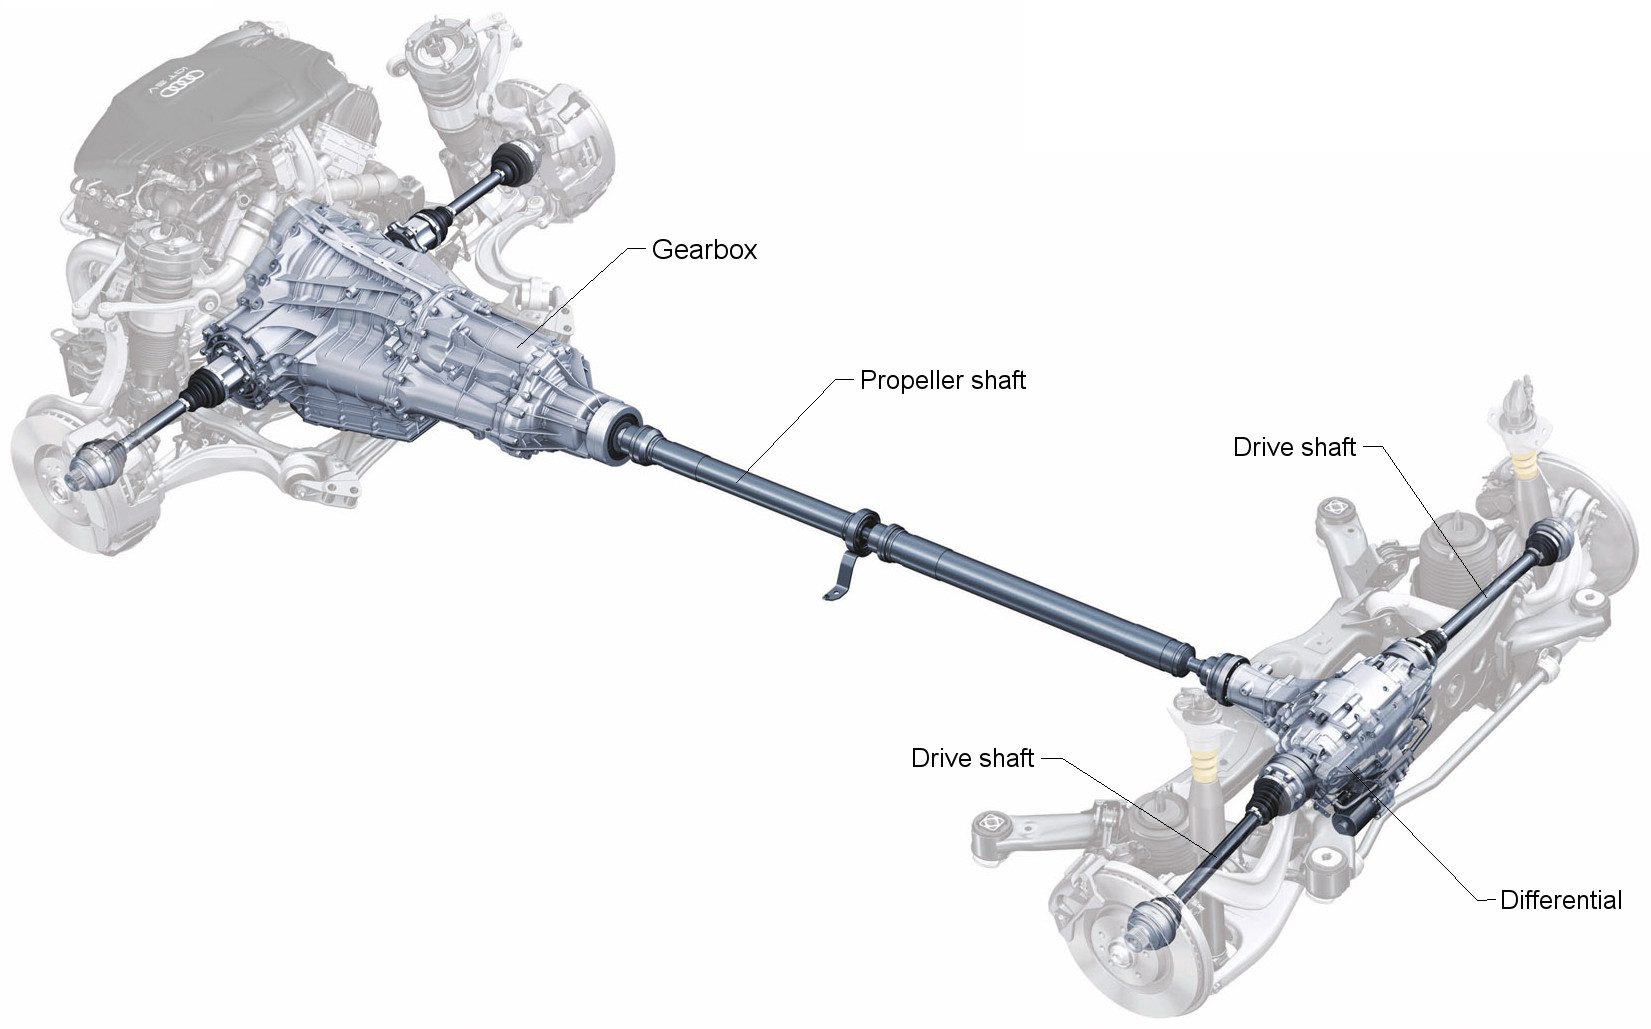
\includegraphics[width=3.5in]{images/fig1.jpg}
\caption{Motion transfer mechanism of an automobile, Taken from \cite{takawane_2019_car}}
\label{fig1}
\end{figure}

\begin{figure}[!t]
\centering
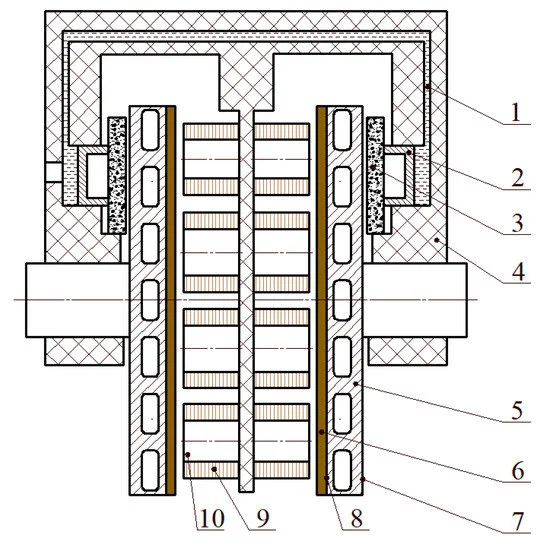
\includegraphics[width=3.5in]{images/fig2.png}
\caption{Structural diagram of the electromagnetic-frictional integrated brake. 1, brake fluid; 2, brake piston; 3, brake pad; 4, caliper body; 5, integrated brake disc; 6, copper layer; 7, friction brake surface; 8, electromagnetic brake surface; 9, coil; and 10, iron core, Taken from \cite{wang_2019_performances}}
\label{fig2}
\end{figure}
Most ECBS \cite{putra_2021_mini,gulec_2016_design,shi_2013_study,shi_2013_study} utilize electromagnets to induce eddy currents in the rotor. Other systems use PM \cite{fontchastagner_2017_axialfield,fontchastagner_2018_design,shin_2013_analytical}to simplify construction but these systems then require complex control systems. An alternative is DC current assisted PM braking where an electromagnet is created by a dc current to short the flux paths as shown in \ref{fig3}. 
\begin{figure}[!t]
\centering
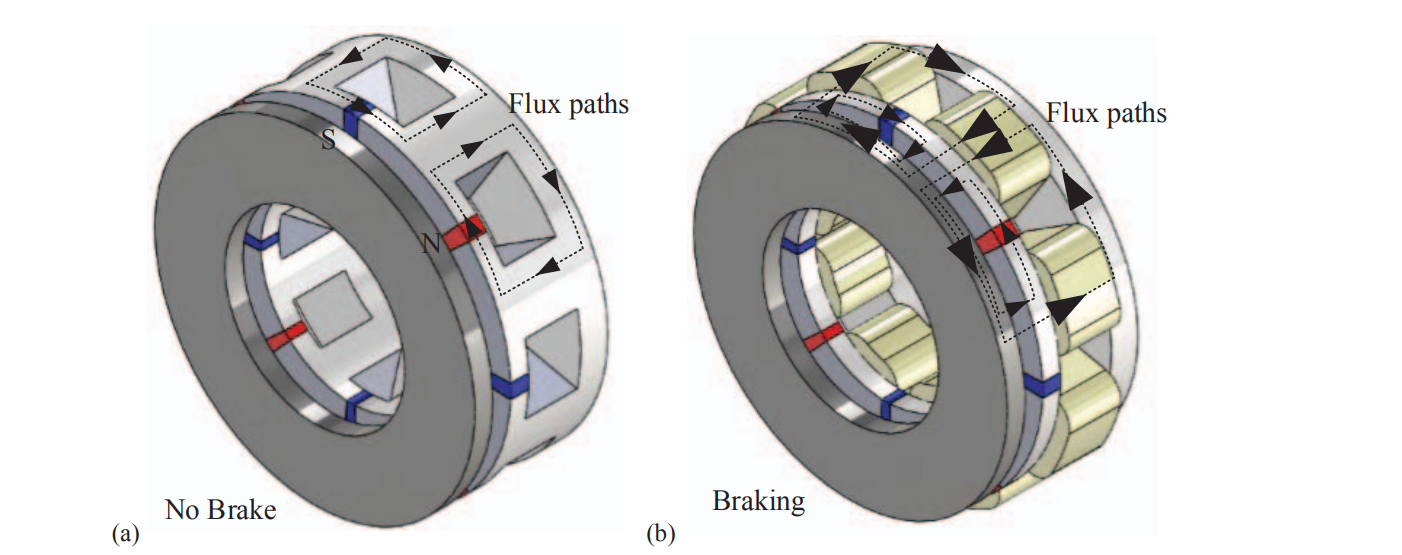
\includegraphics[width=3.5in]{images/fig3.png}
\caption{Motion transfer mechanism of an automobile, Taken from \cite{takawane_2019_car}}
\label{fig3}
\end{figure}

\subsection{Aims, Objectives and Scope}
The hybrid system should provide a 20\% reduction in heating compared to the friction braking system and should produce at least 1200Nm of torque for 800RPM(a little over 100kmh) and should offer a speed reduction of 50\% in the first 25s.
\subsection{Outline of Paper}

\section{Background Theory}
\section{Related Work}
\section{Methodology}
\section{Results}
\section{Conclusion}
The files and models from the stuy can be found at the author' s repository\footnote[1]{https://github.com/shanks847/Axial-Flux-Permanent-Magnet-Eddy-Current-Brake}
\bibliographystyle{IEEEtran}
\bibliography{refs}


\end{document}


